\section[Расчётная часть]{РАСЧЁТНАЯ ЧАСТЬ}

\subsection{Описание комплекса технических средств системы}

Проектируемое приложение предназначено для использования
на мобильных устройствах под управлением операционной системы Android
версии не ниже 4.0.1.

Для полноценной работы приложения требуется наличие фотокамеры.

\subsection{Организация работы системы}

Рассмотрим несколько диаграмм, разработанных по методологиям IDEF0 и IDEF3,
описывающих работу проектируемого приложения.

% main
На рисунке~\ref{fig:idef0_main} представлена диаграмма декомпозиции
верхнего уровня.

\begin{figure}[h!]
  \centering
  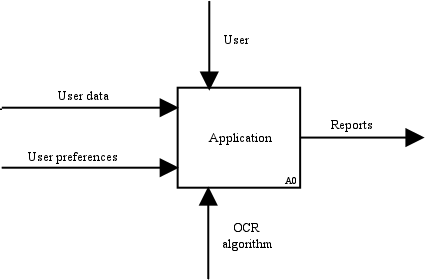
\includegraphics[width=130mm]{pic/idef0_main}
  \caption{Диаграмма декомпозиции \\ верхнего уровня}
  \label{fig:idef0_main}
\end{figure}

Из этой диаграммы видно, что входом системы служат финансовые данные пользователя,
а также его личные предпочтения,
результатом работы системы являются финансовые отчёты,
роль механизма выполняет алгоритм распознавания изображений (OCR),
а управление осуществляет пользователь приложения.

\pagebreak
% application
На рисунке~\ref{fig:idef0_app} представлена диаграмма декомпозиции
приложения.

\begin{figure}[h!]
  \centering
  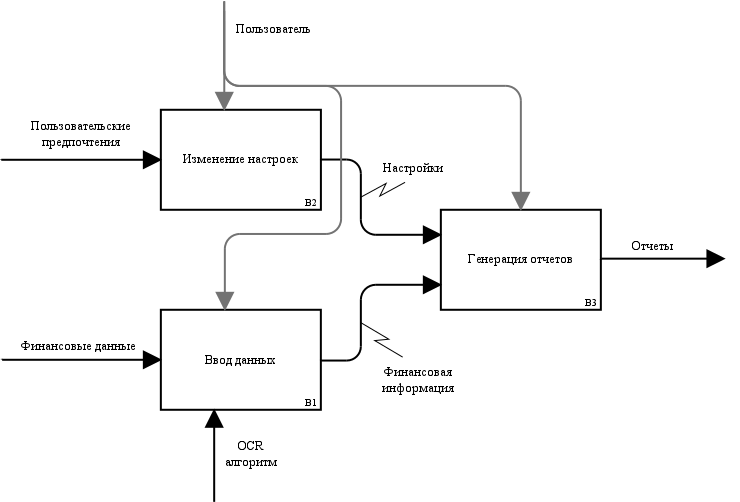
\includegraphics[width=150mm]{pic/idef0_app}
  \caption{Диаграмма декомпозиции приложения}
  \label{fig:idef0_app}
\end{figure}

В соответствии с диаграммой, работу приложения можно разделить
на следующие части:
\begin{itemize}
\item изменение настроек приложения;
\item ввод финансовых данных;
\item генерация отчётов на основании хранимых данных и настроек.
\end{itemize}

Входом для блока <<Изменение настроек>> являются пользовательские
предпочтения, а выходом --- набор настроек, сохраненных в системе.

Финансовые данные, обрабатываемые в блоке <<Ввод данных>>
с использованием алгоритма распознавания изображений,
преобразуются в структурированную финансовую информацию.

Финансовая информация и настройки приложения определяют содержание
отчётов, производимых в блоке <<Генерация отчётов>>.

\pagebreak
% settings
Рассмотрим более подробно схему выбора настроек приложения,
представленную на рисунке~\ref{fig:idef3_settings}.

\begin{figure}[h!]
  \centering
  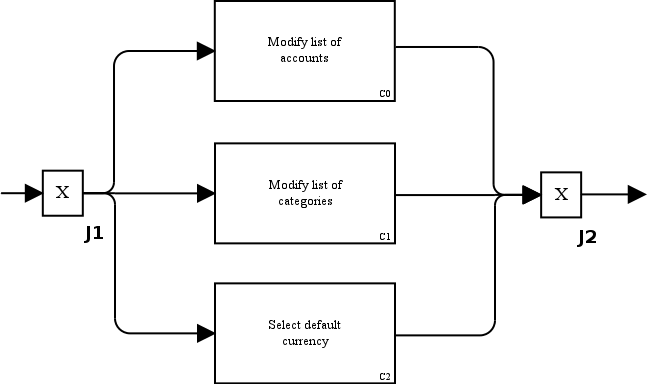
\includegraphics[width=150mm]{pic/idef3_settings}
  \caption{Диаграмма выбора настроек приложения}
  \label{fig:idef3_settings}
\end{figure}

В соответствии с ней, пользователь имеет возможность
добавить или удалить финансовый счёт,
изменить список категорий учета денежных средств,
а также выбрать валюты ввода и представления финансовых
данных по умолчанию.

\pagebreak
% input
Рассмотрим диаграмму процесса ввода данных,
представленную на рисунке~\ref{fig:idef3_input}.

\begin{figure}[h!]
  \centering
  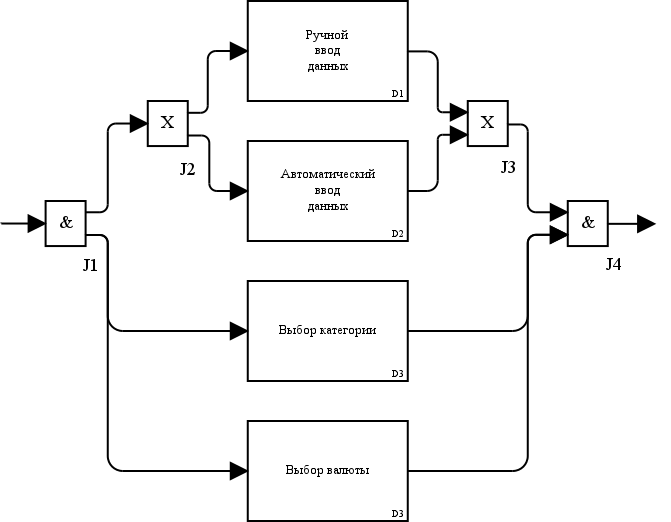
\includegraphics[width=150mm]{pic/idef3_input}
  \caption{Диаграмма процесса ввода данных}
  \label{fig:idef3_input}
\end{figure}

В соответствии с ней, пользователь может вводить числовые данные
вручную, либо с помощью фотокамеры; выбирать выбрать категорию учета,
а также дату ввода.


\pagebreak
% input
Наконец, рассмотрим процесс получения финансовых отчётов,
представленный на рисунке~\ref{fig:idef3_reports}.

\begin{figure}[h!]
  \centering
  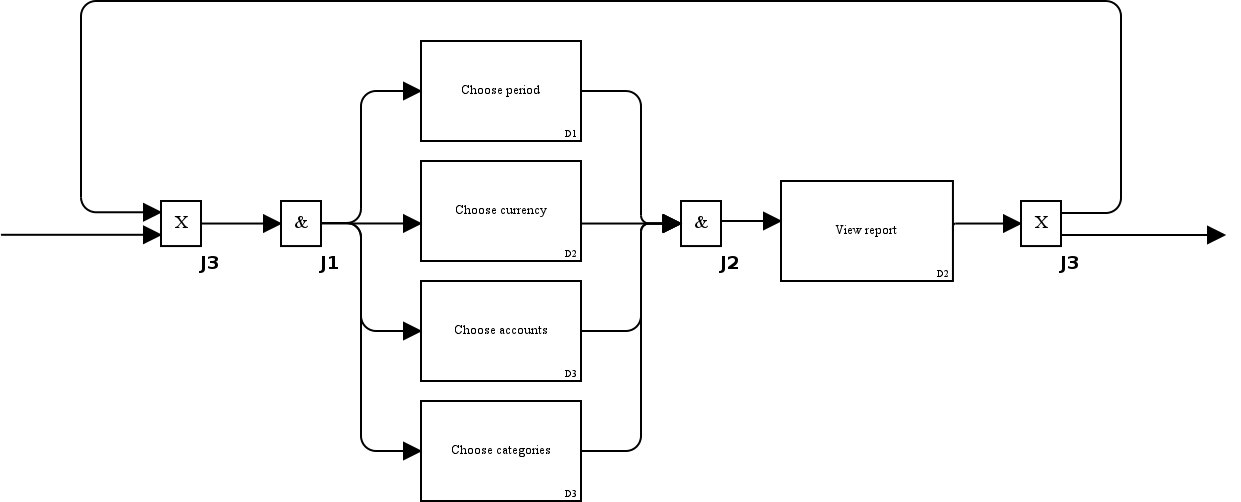
\includegraphics[width=150mm]{pic/idef3_reports}
  \caption{Диаграмма процесса получения отчёта}
  \label{fig:idef3_reports}
\end{figure}

В соответствии с представленной диаграммой, для получения
финансового отчёта пользователь должен выбрать финансовый счёт,
категории учета, а также учетный период.
На основании этих предпочтений пользователя, а также информации
об изменении финансового состояния пользователя,
хранящейся в базе данных, система предоставит требуемый финансовый отчёт.

\pagebreak
\subsection{Пользовательский интерфейс системы}

В данном разделе будет рассмотрен дизайн интерфейса системы с точки зрения
конечного пользователя.

Приложения, разрабатываемые для мобильных платформ, можно разделить
на экраны --- различные части приложения, выполняющие предопределенную роль.

Примерами таких экранов для проектируемого приложения являются:
\begin{itemize}
\item главный экран;
\item экран ввода данных;
\item экран вывода состояния счёта.
\end{itemize}

На рисунке~\ref{fig:screen_main} представлен эскиз макета главного экрана приложения.

\begin{figure}[h!]
  \centering
  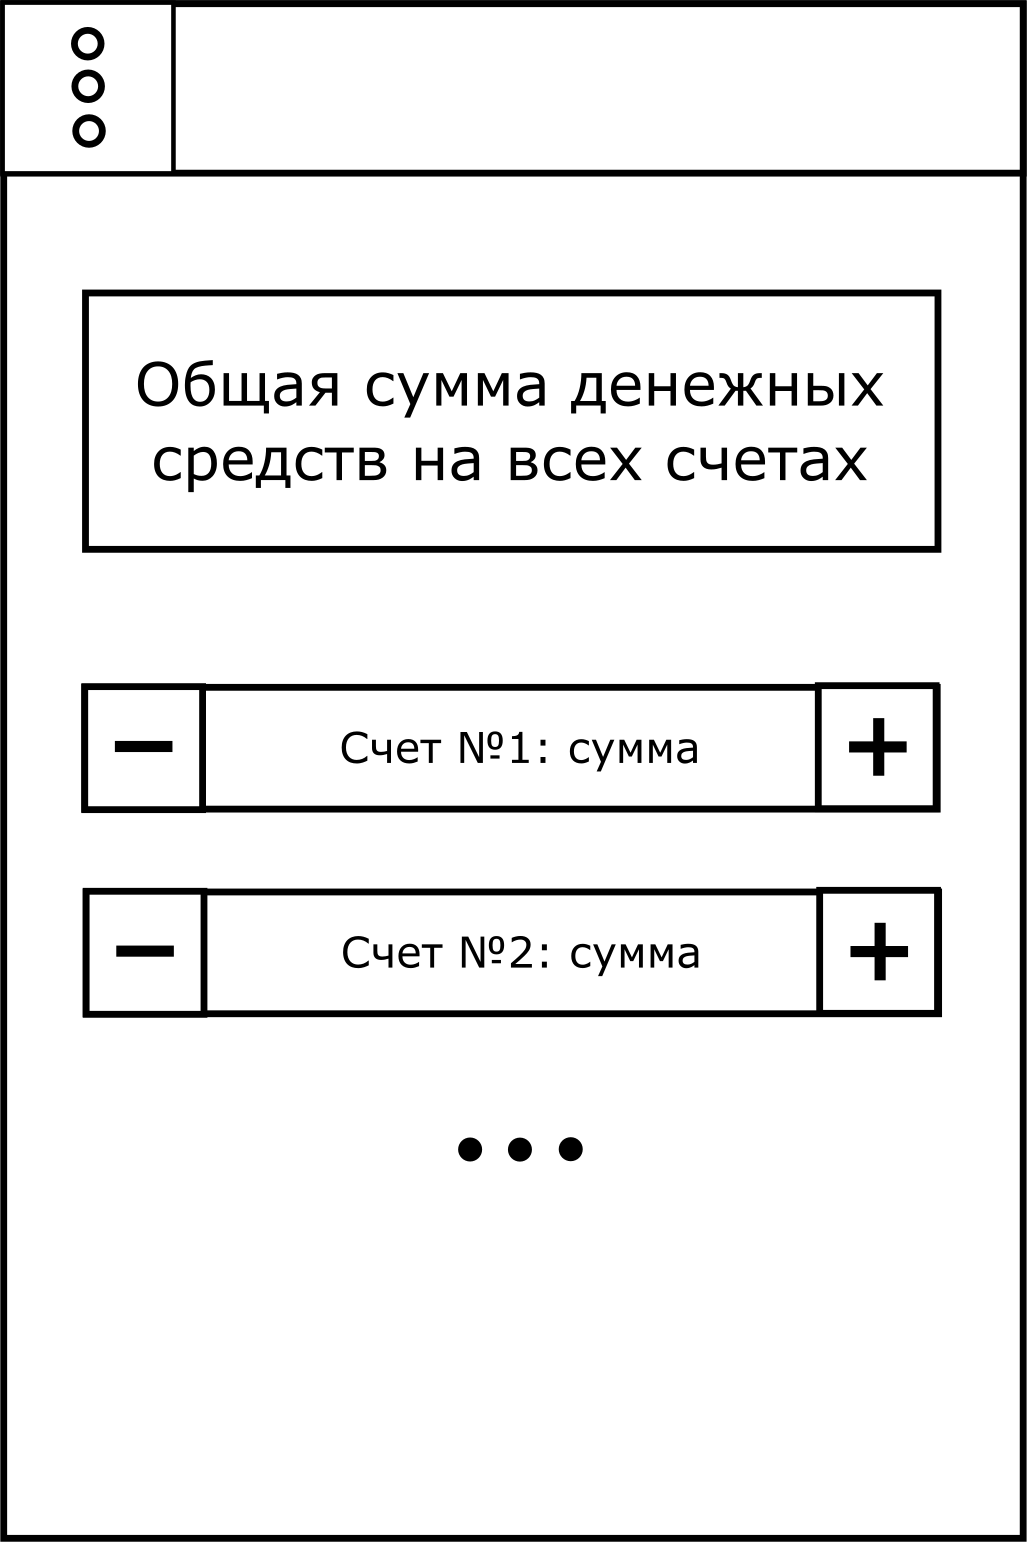
\includegraphics[width=60mm]{pic/screen_main}
  \caption{Главный экран приложения}
  \label{fig:screen_main}
\end{figure}

Он отображает общий баланс денежных средств пользователя,
а также предоставляет возможность ввода финансовых данных для
выбранного счёта (например, <<Работа>>, <<Стипендия>>, и~т.~п.).

По нажатию на общую сумму денежных средств производится переход на
экран вывода общего состояния счётов.
По нажатию на названию счёта производится переход на
экран вывода состояния выбранного счёта.
По нажатию на кнопку <<плюс>> или <<минус>> производится переход на
экран ввода финансовых данных для выбранного счёта.

На рисунке~\ref{fig:screen_input} представлен эскиз макета экрана ввода данных.

\begin{figure}[h!]
  \centering
  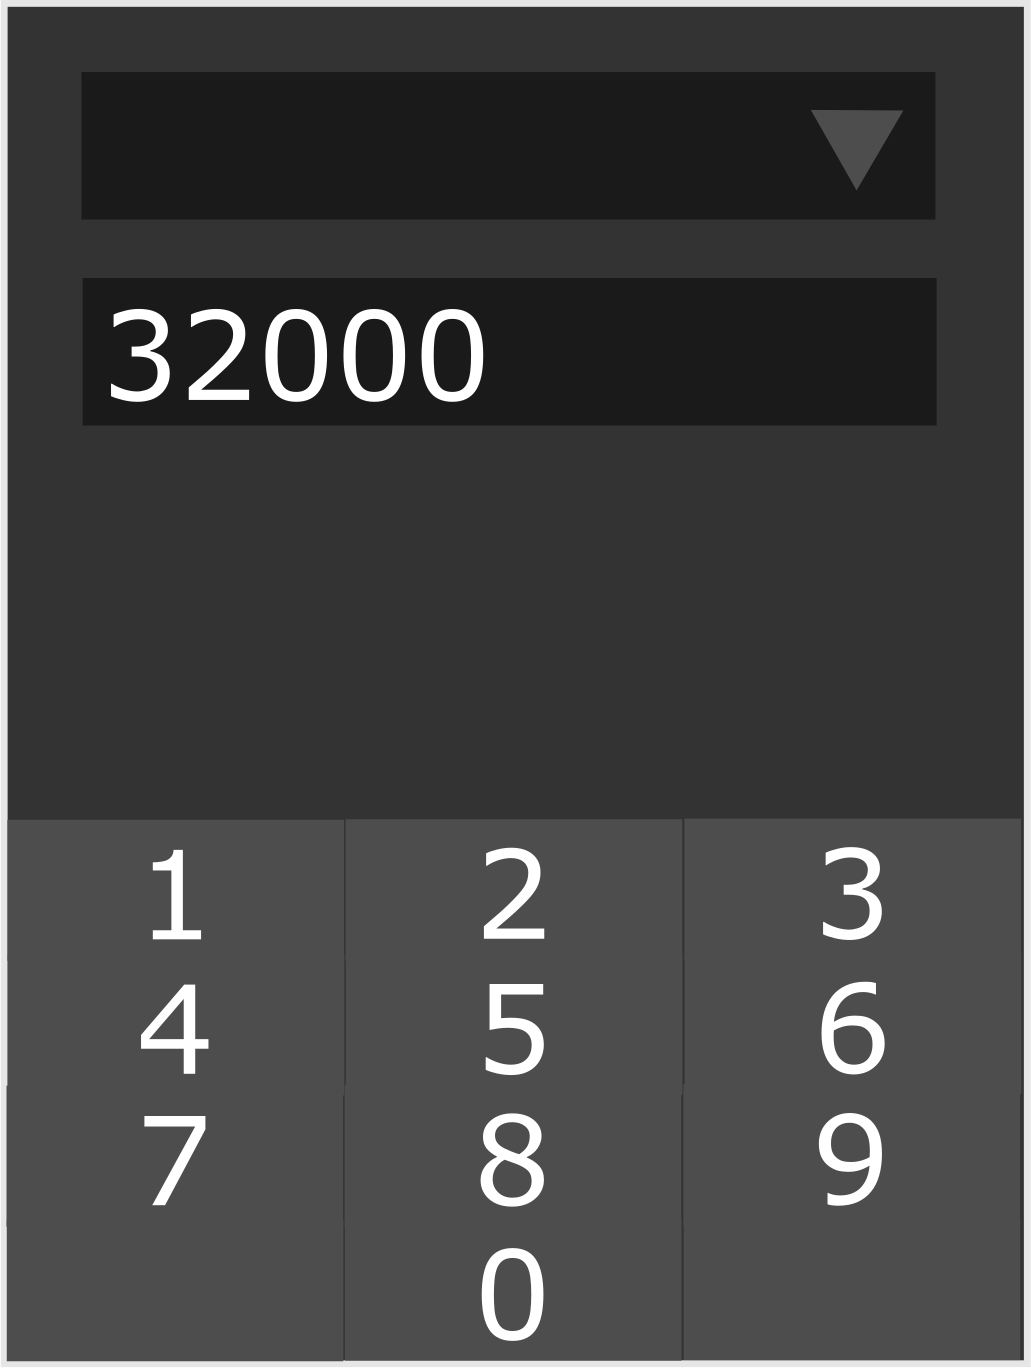
\includegraphics[width=130mm]{pic/screen_input}
  \caption{Экран ввода данных}
  \label{fig:screen_input}
\end{figure}

При нажатии на область ввода значения автоматически появляется клавиатура,
с помощью которой пользователь может ввести требуемую сумму.
При нажатии на кнопку <<P>> запускается модуль, который распознает изображение
с фотокамеры и заполняет поле ввода автоматически.
Далее пользователь может выбрать категорию учета,
нажав на соответствующий элемент интерфейса.

\pagebreak
На рисунке~\ref{fig:screen_reports} представлен эскиз макета экрана состояния
счёта пользователя.

\begin{figure}[h!]
  \centering
  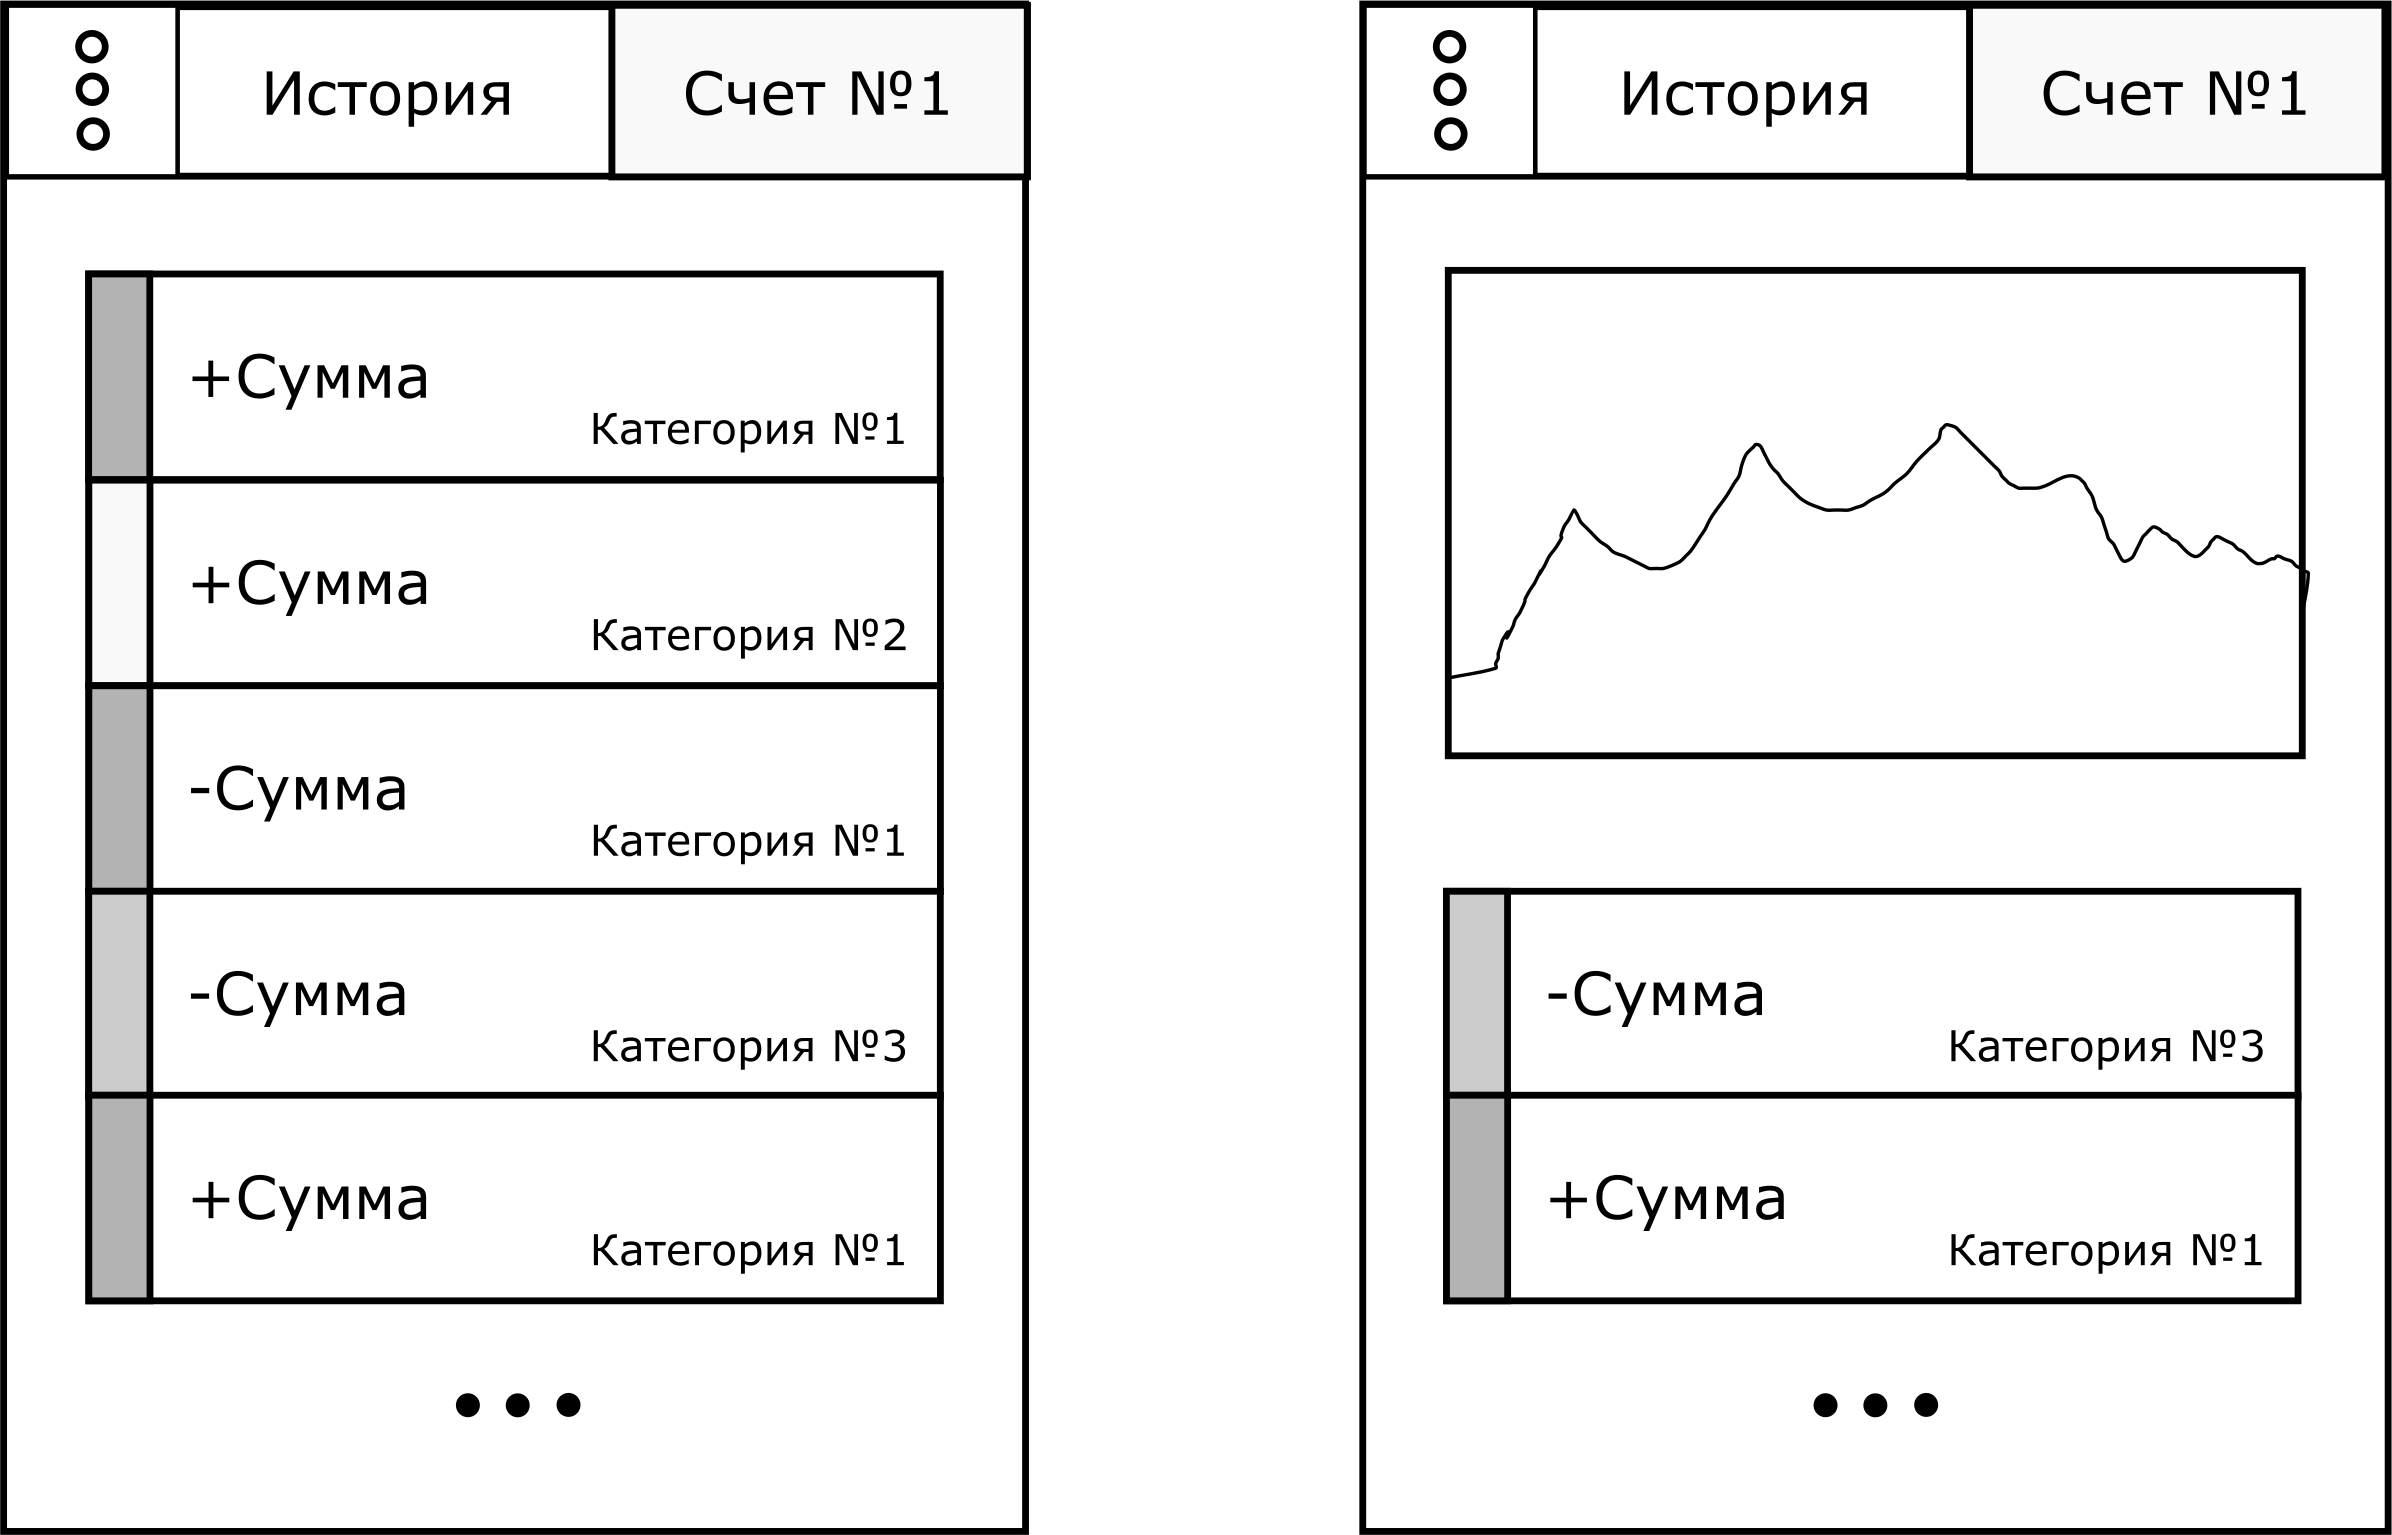
\includegraphics[width=130mm]{pic/screen_reports}
  \caption{Экран вывода состояния счёта}
  \label{fig:screen_reports}
\end{figure}

Он содержит список записей об изменении состояния выбранного счёта,
а также график изменения его баланса.
Каждая запись содержит значение изменения состояния счёта, категорию
учета, отмеченную названием, а также условным цветом заливки (слева).
Имеется возможность выбрать конкретный счет для просмотра, а также
получить общий отчет по счетам, нажав на кнопку <<Счет №1>>
в верхнем правом углу экрана.

\pagebreak
На рисунке~\ref{fig:screen_settings} представлен эскиз макета экрана
настроек приложения.

\begin{figure}[h!]
  \centering
  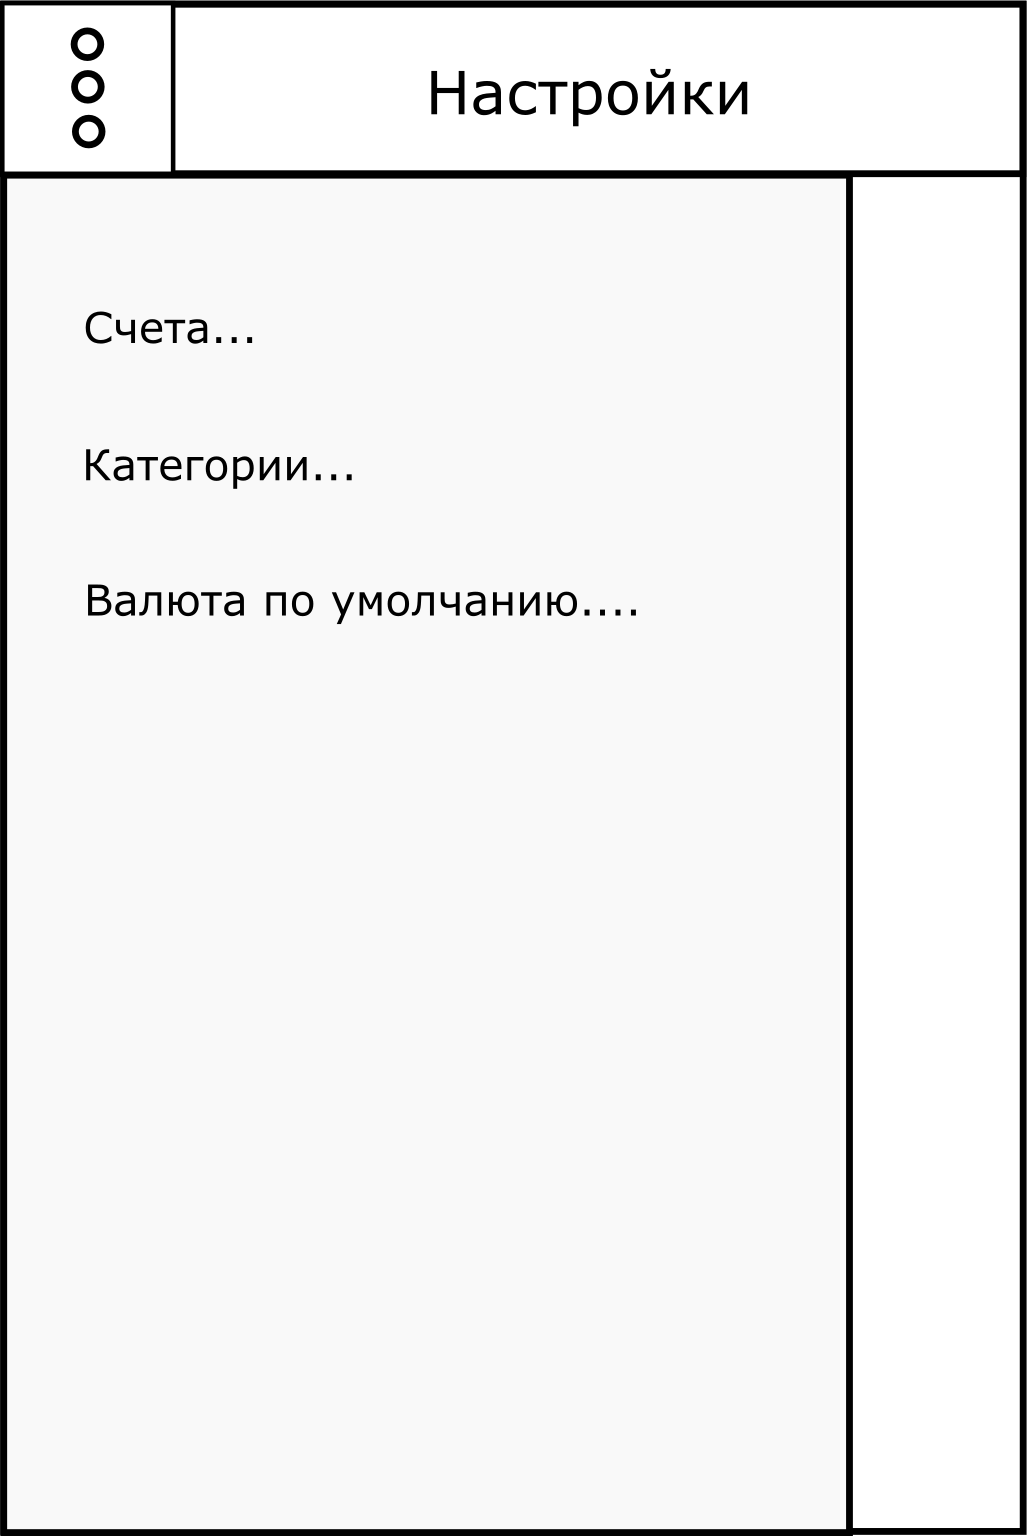
\includegraphics[width=60mm]{pic/screen_settings}
  \caption{Экран настроек приложения}
  \label{fig:screen_settings}
\end{figure}

Он открывается путем нажатия на кнопку, расположенную в
левом верхнем углу каждого экрана приложения.
С помощью него можно выполнить редактирование списка счетов
(выбрать название и валюту счета),
категорий (выбрать название и условный цвет)
а также валюту ввода по умолчанию.